\chapter{Algoritmy násobení matic}

\section{Podle definice}

Základním algoritmem násobení dvou matic je podle definice. Ve třech for cyklech postupně  vybíráme řádky matice A, sloupce matice B a v N krocích násobíme. N je jak šírka matice A, tak i výška matice B.

\begin{algorithm}
	\caption{Násobení matic podle definice}\label{mmm-by-definiton}
	\begin{algorithmic}[1]
		\Procedure{MMM-definition}{$A,B,C$}\Comment{A,B,C jsou matice}
\For{\texttt{$row\gets0$\TO$A.height$}}\Comment{řádky}
	\For{\texttt{$col\gets0$\TO$B.width$}}\Comment{sloupce}
		\State \texttt{$sum \gets 0;$}
		\For{\texttt{$i\gets0$\TO$A.height$}}
			\State \texttt{$sum \gets sum + A[row][i] * B[i][col];$}
		\EndFor
		\State \texttt{$C[row][col] \gets sum;$}
	\EndFor
\EndFor
		\EndProcedure
	\end{algorithmic}
\end{algorithm}

Z pseudokódu je vidět, že ve dvou for cyklech provádíme $N$ násobení a $N$ sčítaní. Asymptotická složitost je tedy $O(n^2(n + n))$ = $O(2n^3)$. V ukázkových výpočtech je násobení pouze $N-1$ krát, to proto, že neuvádíme přičítání k nule (řádek 6).

%%%%%%%%%%%%%%%%%%%%%%%%%%%%%%%%%%%%%%%%%%%%%%%%%%%%%%%%%%%%%%%%%%%%%%%%%%%%%%%%%%%%

\section{Násobení transponovanou maticí}

Pokud nám formát uložení matice nedovolí procházet prvky po sloupcích, je řešením druhou matici transponovat. Poté můžeme násobit řádky matice A s řádky transponované matice B.

\begin{algorithm}
	\caption{Násobení transponovanou maticí}\label{mmm-transpose}
	\begin{algorithmic}[1]
		\Procedure{MMM-transpose}{$A,B,C$}\Comment{A,B,C jsou matice}
\State \texttt{$B \gets transpose(B)$}
\For{\texttt{$rowA\gets0$\TO$A.height$}}\Comment{řádky}
	\For{\texttt{$rowB\gets0$\TO$B.height$}}\Comment{sloupce}
		\State \texttt{$sum \gets 0;$}
		\For{\texttt{$i\gets0$\TO$A.height$}}
			\State \texttt{$sum \gets sum + A[rowA][i] * B[i][rowB];$}
		\EndFor
		\State \texttt{$C[rowA][rowB] \gets sum;$}
	\EndFor
\EndFor
		\EndProcedure
	\end{algorithmic}
\end{algorithm}

Podobný algoritmus můžeme použít i~pokud nám formát nedovolí procházet prvky po řádcích, ale pouze po sloupcích. Například v této práci neuvedený Compressed Sparse Columns.

%XXX: Pro matice musí platit, že výška matice A musí být stejná jako výška matice B. (FIXME: je to opravdu tak?)

%%%%%%%%%%%%%%%%%%%%%%%%%%%%%%%%%%%%%%%%%%%%%%%%%%%%%%%%%%%%%%%%%%%%%%%%%%%%%%%%%%%%

\section{Násobení po řádcích}

Další možností jak násobit dvě matice, kde nám formát uložení nedovolí procházet po sloupcích je procházet současně řádky matice A i B a přičítat jednotlivé součiny na správné místo ve výsledné matici C.

Nevýhodou tohoto řešení je velký počet přístupů do pole C. Protože k~prvkům přičítáme, tedy načítáme a sčítáme, je potřeba před samotným násobením nastavit všechny prvky matice C na hodnotu nula.

%tohle neplati: Matice musí být stejně široké i vysoké.

\begin{algorithm}
	\caption{Násobení po řádcích}\label{mmm-by-rows}
	\begin{algorithmic}[1]
		\Procedure{MMM-by-rows}{$A,B,C$}\Comment{A,B,C jsou matice}
\For{\texttt{$r\gets0$\TO$A.height$}}\Comment{řádky matice A i B}
	\For{\texttt{$cA\gets0$\TO$A.width$}}\Comment{sloupce matice A}
		\For{\texttt{$cB\gets0$\TO$B.width$}}\Comment{sloupce matice B}
			\State \texttt{$C[r][cA] \gets C[r][cA] + A[r][cA] * B[r][cB];$}
		\EndFor
	\EndFor
\EndFor
		\EndProcedure
	\end{algorithmic}
\end{algorithm}

%%%%%%%%%%%%%%%%%%%%%%%%%%%%%%%%%%%%%%%%%%%%%%%%%%%%%%%%%%%%%%%%%%%%%%%%%%%%%%%%%%%%

\section{Rekurzivní násobení}

Pro matice A i B o stejé velikosti $ {2^\mathbf{N}} $ můžeme použít rekurzivní přístup. Tedy programovací techniku rozděl a panuj, kdy rozdělíme větší problémy na menší podproblémy.

Každou z matic rozdělíme na čtvrtiny a jednotlivé podmatice násobíme algoritmem podle definice, tedy jako matice o velikosti dva.

\label{2x2MMM}
\begin{align}
\begin{pmatrix}
 a & b \\
 c & d
\end{pmatrix} \cdot \begin{pmatrix}
 e & f \\
 g & h
\end{pmatrix} = \begin{pmatrix}
 ae+bg & af+bh \\
 ce+dg & cf+dh
\end{pmatrix}
\end{align}

Tento postup opakujeme, dokud velikostí podmatic nenarazíme na práh, tedy hodnotu, při které opustíme rekurzivní algoritmus a použijeme algoritmus lineární. V ukázkovém pseudokódu dělíme podmatice až na velikost prahu jedna, podmatice tedy obsahují pouze jeden prvek.

\begin{algorithm}[H]
	\caption{Rekurzivní násobení}\label{mmm-recursive}
	\begin{algorithmic}[1]
		\Procedure{MMM-recursive}{$A,B,C,ay,ax,by,bx,cy,cx,n$}
		\If{$n = 1$}
			\State \texttt{$C[cy][cx]\gets C[cy][cx] + A[ay][ax] \cdot B[by][bx];$}
			\State \texttt{$return;$}
		\EndIf
		\ForAll{\texttt{$r \in \{ 0, n/2 \}$}}
			\ForAll{\texttt{$c \in \{ 0, n/2 \}$}}
				\ForAll{\texttt{$i \in \{ 0, n/2 \}$}}
					\State \texttt{MMM-recursive$(A,B,C,ay+i,ax+r,by+c,bx+i,cy+c,cx+r,n/2);$}
				\EndFor
			\EndFor
		\EndFor
		\EndProcedure
	\end{algorithmic}
\end{algorithm}

Pro ilustraci jako příklad uvádíme výpočet horního levého prvku v násobení dvou matic o velikosti $ 2^{2} $. Pro větší přehlednost značíme prvky malým písmem z názvu matice a indexy o jejich pozicích.

\begin{align}
\begin{pmatrix}
a_{1,1} & a_{1,2} & a_{1,3} & a_{1,4} \\
a_{2,1} & a_{2,2} & a_{2,3} & a_{2,4} \\
a_{3,1} & a_{3,2} & a_{3,3} & a_{3,4} \\
a_{4,1} & a_{4,2} & a_{4,3} & a_{4,4}
\end{pmatrix} \cdot \begin{pmatrix}
b_{1,1} & b_{1,2} & b_{1,3} & b_{1,4} \\
b_{2,1} & b_{2,2} & b_{2,3} & b_{2,4} \\
b_{3,1} & b_{3,2} & b_{3,3} & b_{3,4} \\
b_{4,1} & b_{4,2} & b_{4,3} & b_{4,4}
\end{pmatrix} = \\
\begin{pmatrix}
%----------------------------------------
\begin{pmatrix}
 a_{1,1} & a_{1,2} \\
 a_{2,1} & a_{2,2} \\
\end{pmatrix} \cdot
\begin{pmatrix}
 b_{1,1} & b_{1,2} \\
 b_{2,1} & b_{2,2} \\
\end{pmatrix} + 
\begin{pmatrix}
 a_{1,3} & a_{1,4} \\
 a_{2,3} & a_{2,4} \\
\end{pmatrix} \cdot 
\begin{pmatrix}
 b_{3,1} & b_{3,2} \\
 b_{4,1} & b_{4,2} \\
\end{pmatrix} &
\hdots \\
\hdots & \hdots
\end{pmatrix} = \\
\begin{pmatrix}
%----------------------------------------
\begin{pmatrix}
 a_{1,1} b_{1,1}+a_{1,2} b_{2,1} & \hdots \\
 \hdots & \hdots
\end{pmatrix} + 
\begin{pmatrix}
 a_{1,3} b_{3,1}+a_{1,4} b_{4,1} & \hdots \\
 \hdots & \hdots
\end{pmatrix} &
\hdots \\
\hdots & \hdots
\end{pmatrix} = \\
\begin{pmatrix}
\begin{pmatrix}
 a_{1,1} b_{1,1}+a_{1,2} b_{2,1}+a_{1,3} b_{3,1}+a_{1,4} b_{4,1} & \hdots \\
\hdots & \hdots
\end{pmatrix} &
\hdots \\\hdots & \hdots
\end{pmatrix}
\end{align}


Kvůli režii rekurzivního dělení v praxi nezmenšujeme podmatice až na velikost jedna. Vhodný práh velikosti podmatice je například takový, co se vejde do L1 cache.

Asymptotická složitost je samozřejmě stejná jako u algoritmu podle definice. Asymptotickou složitost rekurzivního algoritmu můžeme spočítat pomocí mistrovské metody.

\[ T(n) = \left\{ 
  \begin{array}{l l}
    \Theta(1) & \quad \text{if $n$ = 1}\\
    8T(n/2) + \Theta(1) & \quad \text{if $n$ > 1}
  \end{array} \right.\]

Protože platí, že $a=8, b=2, r=\log_{2} 8, n^r=n^{\log_{2} 8}=n^3=\Omega(1)$, tak asymptotická složitost podle mistrovké metody je \texttt{MMM-recursive}(n) = $O(n^3)$.

%%%%%%%%%%%%%%%%%%%%%%%%%%%%%%%%%%%%%%%%%%%%%%%%%%%%%%%%%%%%%%%%%%%%%%%%%%%%%%%%%%%%%%%%%%%%%%%%%%%%%%%%%%%%%%%%%%%%%%%%%%%%%%%%
\section{Strassenův algoritmus} %%%%%%%%%%%%%%%%%%%%%%%%%%%%%%%%%%%%%%%%%%%%%%%%%%%%%%%%%%%%%%%%%%%%%%%%%%%%%%%%%%%%%%%%%%%%%%%%

V roce 1969 Volker Strassen v časopise Numerische Mathematik publikoval článek \cite{GEMnO}, ve kterém jako první představil algoritmus násobení dvou matic s menší asymptotickou složitostí než algotimus podle definice, tedy $O(n^3)$.

Algoritmus je založen na myšlence, že sčítání je operace méně náročnejší než operace násobení. Respektive dvě matice umíme sečíst nebo odečíst v složitosti $O(n^2)$, ale vynásobit v $O(n^3)$.

Volker Strassen tedy využil jisté symetrie \cite{StrNat} v násobení dvou matic $A$ a $B$ o velikosti dva a výslednou matici $C$ seskládal pomocí sedmi pomocných matic. Obrázek \ref{fig:StrVis} ukazuje, z čeho se pomocné matice skládají a jak jsou do výsledné matice seskládany. V ilustračních maticích o velikosti čtyři ukazujeme, které sčítance pomocná matice do výsledku přičítá a které odečítá. 

\begin{figure}[H]\centering
	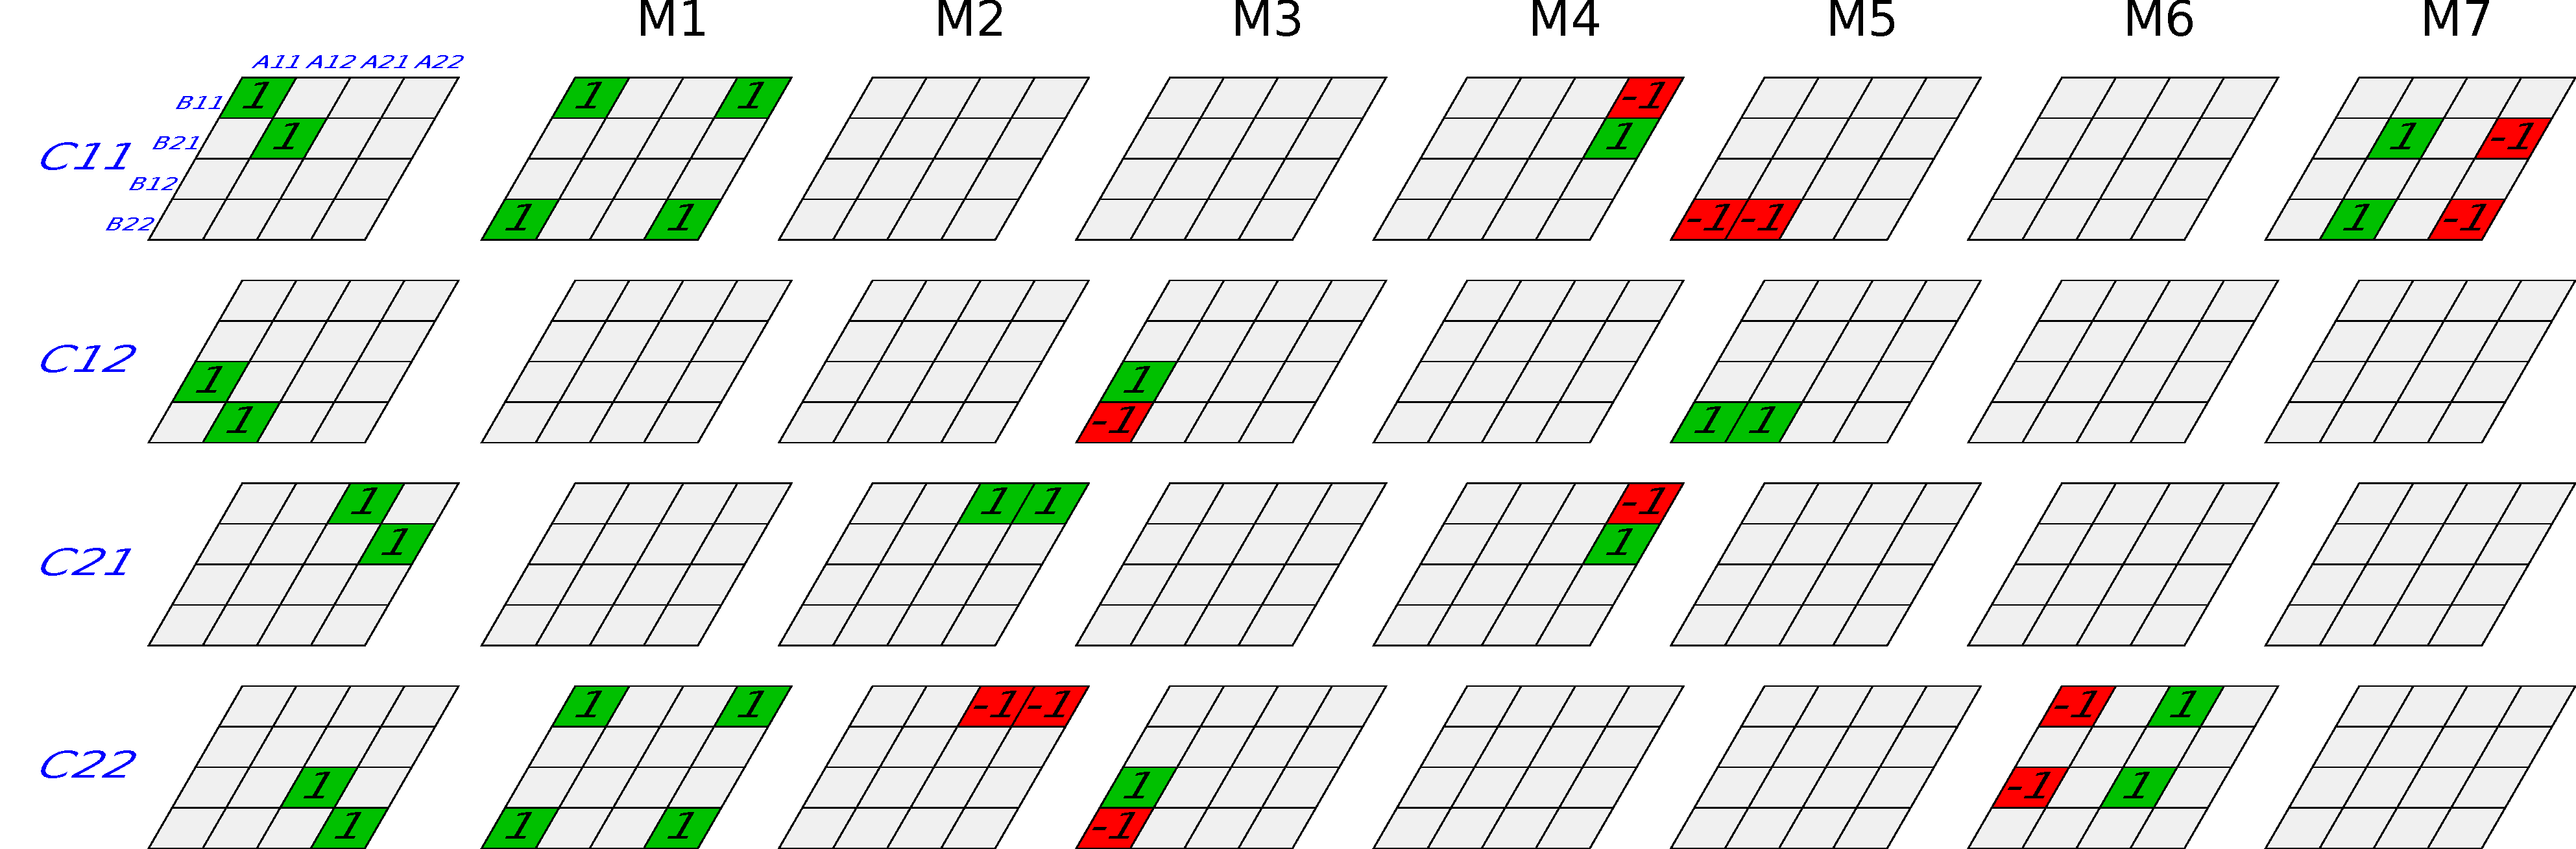
\includegraphics[width=\textwidth]{./images/strassen}
	\caption{Strassen (TODO: převzato z wikipedie: předělat?)}
	\label{fig:StrVis}
\end{figure}

Zápis Strassenova algoritmu vypadá následnovně:	

\begin{align}
A \cdot B = \begin{pmatrix}
 A_{1,1} & A_{1,2} \\
 A_{2,1} & A_{2,2} \\
\end{pmatrix} \cdot \begin{pmatrix}
 B_{1,1} & B_{1,2} \\
 B_{2,1} & B_{2,2} \\
\end{pmatrix} \\
M_{1} = (A_{1,1} + A_{2,2}) \cdot (B_{1,1} + B_{2,2}) \\
M_{2} = (A_{2,1} + A_{2,2}) \cdot B_{1,1} \\
M_{3} = A_{1,1} \cdot (B_{1,2} - B_{2,2}) \\
M_{4} = A_{2,2} \cdot (B_{2,1} - B_{1,1}) \\
M_{5} = (A_{1,1} + A_{1,2}) \cdot B_{2,2} \\
M_{6} = (A_{2,1} - A_{1,1}) \cdot (B_{1,1} + B_{1,2}) \\
M_{7} = (A_{1,2} - A_{2,2}) \cdot (B_{2,1} + B_{2,2}) \\
C = \begin{pmatrix}
 M_{1} + M_{4} - M_{5} + M_{7} & M_{3} + M_{5} \\
 M_{2} + M_{4} & M_{1} - M_{2} + M_{3} + M_{6}
\end{pmatrix}
\end{align}

V pseudokódu používáme procedury \texttt{offset-add} respektive \texttt{offset-sub}. Slouží ke sčítání respektive odečítání bloku prvků o velikosti n v maticích od nějakého offsetu \texttt{y} a \texttt{x}. Paremetry obou funkcí jsou: \texttt{offset-*}$(A,B,C,ay,ax,by,bx,cy,cx,n)$. 

\begin{algorithm}[H]
	\caption{Strassenův algoritmus}\label{mmm-strassen}
	\begin{algorithmic}[1]
		\Procedure{MMM-strassen}{$A,B,C,ay,ax,by,bx,cy,cx,n$}
		\If{$n = 1$}
			\State \texttt{$C[cy][cx]\gets C[cy][cx] + A[ay][ax] \cdot B[by][bx];$}
			\State \texttt{$return;$}
		\EndIf
  		\State \texttt{$h \gets n/2;$} \Comment{čtvrtina}
  		\State \texttt{$m[9] \gets $init-matrices$(9, h);$} \Comment{devět pomocných matic}
 % 	
	\State \texttt{offset-add$(a, a, m[8], ay, ax, ay + h, ax + h, 0, 0, h);$} \Comment{M1}
	\State \texttt{offset-add$(b, b, m[9], by, bx, by + h, bx + h, 0, 0, h);$}
	\State \texttt{MMM-strassen$(m[8], m[9], m[1], 0, 0, 0, 0, 0, 0, h);$}
%	
	\State \texttt{offset-add$(a, a, m[8], ay + h, ax, ay + h, ax + h, 0, 0, h);$} \Comment{M2}
	\State \texttt{MMM-strassen$(m[8], b, m[2], 0, 0, bx, by, 0, 0, h);$}
%	
	\State \texttt{offset-sub$(b, b, m[8], by, bx + h, by + h, bx + h, 0, 0, h);$} \Comment{M3}
	\State \texttt{MMM-strassen$(a, m[8], m[3], ay, ax, 0, 0, 0, 0, h);$}
%	
	\State \texttt{offset-sub$(b, b, m[8], by + h, bx, by, bx, 0, 0, h);$} \Comment{M4}
	\State \texttt{MMM-strassen$(a, m[8], m[4], ay + h, ax + h, 0, 0, 0, 0, h);$}
%	
	\State \texttt{offset-add$(a, a, m[8], ay, ax, ay, ax + h, 0, 0, h);$} \Comment{M5}
	\State \texttt{MMM-strassen$(m[8], b, m[5], 0, 0, by + h, bx + h, 0, 0, h);$}
%	
	\State \texttt{offset-sub$(a, a, m[8], ay + h, ax, ay, ax, 0, 0, h);$} \Comment{M6}
	\State \texttt{offset-add$(b, b, m[9], by, bx, by, bx + h, 0, 0, h);$}
	\State \texttt{MMM-strassen$(m[8], m[9], m[6], 0, 0, 0, 0, 0, 0, h);$}
%	
	\State \texttt{offset-sub$(a, a, m[8], ay, ax + h, ay + h, ax + h, 0, 0, h);$} \Comment{M7}
	\State \texttt{offset-add$(b, b, m[9], by + h, bx, by + h, bx + h, 0, 0, h);$}
	\State \texttt{MMM-strassen$(m[8], m[9], m[7], 0, 0, 0, 0, 0, 0, h);$}
%	
	\State \texttt{offset-add$(m[1], m[4], m[8], 0, 0, 0, 0, 0, 0, h);$} \Comment{c1,1}
	\State \texttt{offset-sub$(m[8], m[5], m[8], 0, 0, 0, 0, 0, 0, h);$}
	\State \texttt{offset-add$(m[8], m[7], c, 0, 0, 0, 0, cy, cx, h);$}
%	
	\State \texttt{offset-add$(m[3], m[5], c, 0, 0, 0, 0, cy, cx + h, h);$} \Comment{c1,2}
%	
	\State \texttt{offset-add$(m[2], m[4], c, 0, 0, 0, 0, cy + h, cx, h);$} \Comment{c2,1}
%	
	\State \texttt{offset-sub$(m[1], m[2], m[8], 0, 0, 0, 0, 0, 0, h);$} \Comment{c2,2}
	\State \texttt{offset-add$(m[8], m[3], m[8], 0, 0, 0, 0, 0, 0, h);$}
	\State \texttt{offset-add$(m[8], m[6], c, 0, 0, 0, 0, cy + h, cx + h, h);$}		
		\EndProcedure
	\end{algorithmic}
\end{algorithm}


Výpočet asymptotické složitosti vypočteme podobně jako u \texttt{MMM-recursive}, tedy mistrovskou metodou. 

V každém kroku rekurze počítáme $\Theta(n^2)$ operací na vytvoření pomocných matic.

\[ T(n) = \left\{ 
  \begin{array}{l l}
    \Theta(1) & \quad \text{if $n$ = 1}\\
    7T(n/2) + \Theta(n^2) & \quad \text{if $n$ > 1}
  \end{array} \right.\]

Protože platí, že $a=7, b=2, r=\log_{2} 7, n^r=n^{\log_{2} 7}=\Omega(n^2)$, tak asymptotická složitost podle mistrovké metody je \texttt{MMM-strassen}(n) = $O(n^{\log_{2} 7}) \approx O(n^{2.8})$.

Stejně jako v předešlém algorimu, i zde demonstrujeme výpočet levého horního prvku matice z násobení dvou matic o velikosti dva. Místo parametrické matice použijeme konkrétní desetinná čísla, abychom ukázali numerickou stabilitu Strassenova algoritmu. Pro ukázku budeme uvažovat počítač, který u čísel ukládá pouze pět cifer, znaménko a desetinnou čárku.	

Pomocí algoritmu podle definice, by takový počítač vypočítal součin dvou matic následnovně:

\begin{align}
\begin{pmatrix}
 30.234 & 0.5678 \\
 0.9123 & 10.456
\end{pmatrix} \cdot \begin{pmatrix}
 0.8912 & 0.3456 \\
 0.7891 & 9.999 \\
\end{pmatrix} = \begin{pmatrix}
 27.392 & \hdots \\
 \hdots & \hdots
\end{pmatrix}
\end{align}

Správný výsledek je $30.234 \times 0.8912 + 0.5678 \times 0.7891 = 26.9445408 + 0.44805098 = 27.39259178$.

Nyní výpočet provedeme pomocí Strassenova algoritmu:

\begin{align}
\begin{pmatrix}
 30.234 & 0.5678 \\
 0.9123 & 10.456
\end{pmatrix} \cdot \begin{pmatrix}
 0.8912 & 0.3456 \\
 0.7891 & 9.999
\end{pmatrix} \\
M_{1} = (30.234 + 10.456) \cdot (0.8912 + 9.999) = 443.12  \\
\hdots \\
M_{4} = 10.456 \cdot (0.7891 - 0.8912) = -1.067 \\
M_{5} = (30.234 + 0.5678) \cdot 9.999 = 307.98 \\
\hdots \\
M_{7} = (0.5678 - 10.456) \cdot (0.7891 + 9.999) = -106.67 \\
 \begin{pmatrix}
 M_{1} + M_{4} - M_{5} + M_{7} & \hdots \\
 \hdots & \hdots
\end{pmatrix} = \begin{pmatrix}
 27.403 & \hdots \\
 \hdots & \hdots
\end{pmatrix}
\end{align}

% zdroj http://math.nist.gov/MatrixMarket/data/Harwell-Boeing/oilgen/orsirr_1.html

Jak můžeme vidět, zatímco u algoritmu podle definice jsme pouze ztratili desetinnou přesnost, výsledek Strassenova algoritmu se lišil už v prvním desetinném čísle. 

Pro reálnou představu stability Strassenova algoritmu jsme provedli experiment, ve kterém jsme vynásobili dvě stejné matice (matice orsirr\_1, oříznuta na velikost 1024) algoritmem podle definice a Strassenovým algoritmem s různýmy práhy a sečetli všechny rozdíly mezi výsledky. Násobení probíhalo ve dvojté desetinné přesenosti, tedy v datovém typu \texttt{double} jazyka C99. Z grafu \ref{fig:StrassenStability} je vidět exponencionální závislost mezi velikostí prahu a celkovou chybou.

\begin{figure}[H]\centering
	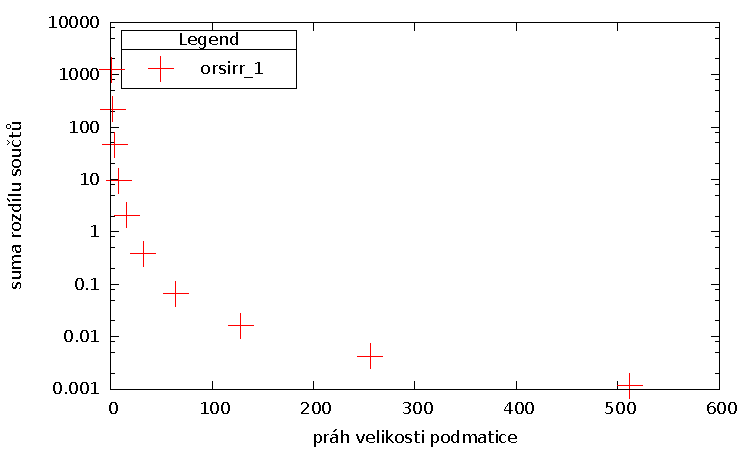
\includegraphics[width=\textwidth]{./images/strassen_stability}
	\caption{Ukázka numerické stability Strassenova algoritmu}
	\label{fig:StrassenStability}
\end{figure}

Strassenův algorimus lze ještě vylepšit. Algoritmům na stejném principu se říká Strassen-like \cite{DBLP:journals/iacr/CenkH13}. Pro sedm operací násobení je monžné snížit počet sčítání a odečítání. Pro jednoduchost zde ovšem uvádíme originalní algoritmus.

\section{Rychlé algoritmy}

Po tom, co Strassen ukázal, že existují rychlejší algoritmy než $O(n^3)$, ještě rychlejší algoritmy než ten jeho na sebe nenechaly dlouho čekat. Složitost násobení matic pro jednoduchost označíme jako $O(n^\omega)$.

Nejpomalejší algoritmus s $\omega=3$ je podle definice. Strassenův algoritmus se sedmi násobeními má $\omega\approx2.807354$. Jeden z nejrychlejších algoritmů je algoritmus Virginie Williamsové \cite{DBLP:conf/stoc/Williams12}\cite{BreakigCWB}, pro který je $\omega<2.3727$. 

Hranicí nejlepší možné složitosti může být $\omega=2$, protože každý prvek z matice musíme nějak započítat. Existují z velké části podložené domněnky na základě teorie grup \cite{complexityMM}, že $\omega=2$ skutečně platí, ale přímý důkaz ještě neexistuje.

\section{Algoritmus podle definice upravený pro řídké matice}

Pokud násobíme řídké matice $A$ a $B$ o velikosti $N$, můžeme vynechat násobení takových dvou prvků, z nichž je alespoň jeden nulový. Označme $nnzr_{M,i}$ jako počet nenulových prvků v i-tém řádku matice M a $nnzc_{M,i}$ jako počet nenulových prvků v i-tém sloupci matice M. Protože násobíme každý řádek s každým sloupcem, bude celkový počet operací násobení dán vzorcem:

\begin{align*}
\sum_{i=1}^{N} nnzr_{A,i} nnzc_{B,i}
\end{align*}

Složitost tohoto algoritmu pro násobení dvou matic $A$ a $B$ o velikosti $n$ tedy můžeme vyjádřit jako $O(mn)$, kde $m = max(nnz(A),nnz(B)$. Pro husté matice bez jediného nulového prvku samozřejmě platí, že $m=n^2$. Nutno podotknout, že $O(mn)$ je nejhorší případ, kdy se všechny nenulové prvky matice $A$ budou násobit se všemy nenulovými prvky matice $B$.

Pro reálnou představu demonstrujeme násobení dvou stejných matic. Opět se jedná o dvě matice orsirr\_1. Matice orsirr\_1 má velikost $n=1030$ a~$m=6858$ nnz. Rozmístění nnz před respektive po vynásobení ukazují obrázky \ref{fig:befOrsirr1} respektive \ref{fig:aftOrsirr1}.

\begin{figure}[H]
	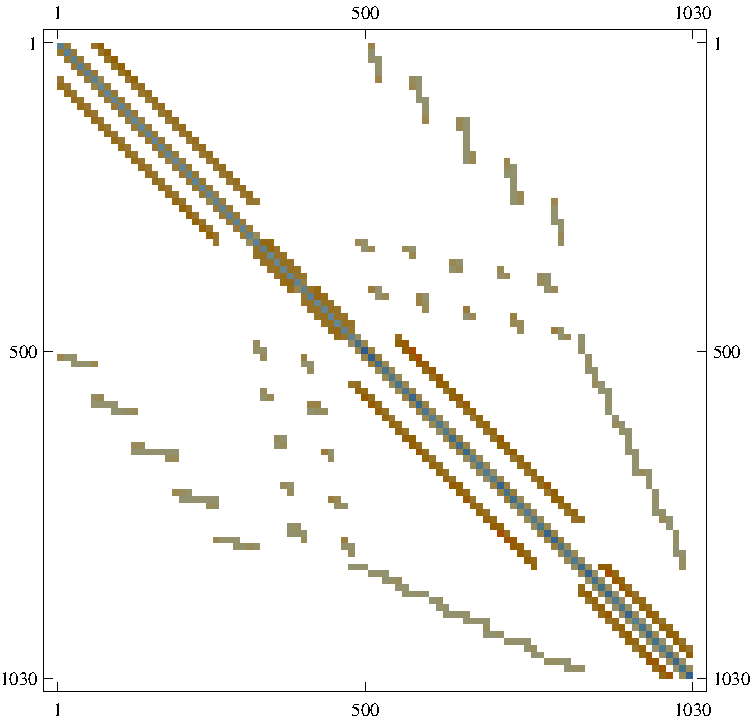
\includegraphics[width=1.0\textwidth]{./images/orsirr_1_orig}
	\caption{Matice orsirr\_1 před vynásobením}
	\label{fig:befOrsirr1}
\end{figure}

\begin{figure}[H]
	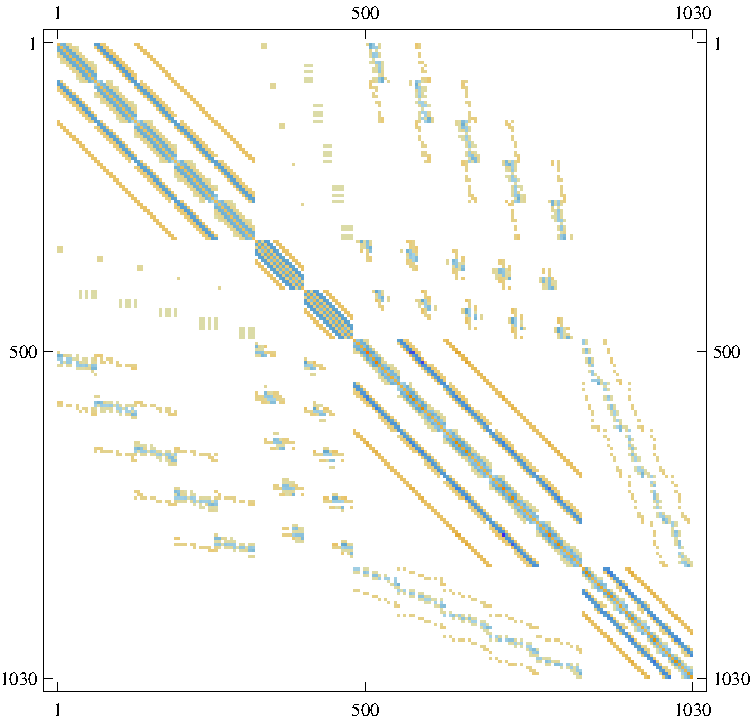
\includegraphics[width=1.0\textwidth]{./images/orsirr_1_mul}
	\caption{Matice orsirr\_1 po vynásobením sama se sebou}
	\label{fig:aftOrsirr1}
\end{figure}

Kdyby nastal nejhorší možný případ, počet operací násobení při použití algoritmu podle definice pro řídké matice by byl $1030 \times 6858 = 7063740$. Pro tento případ ovšem stačí $46976$ operací násobení. Oproti nejhoršímu možnému případu nastalo $7063740 - 46976 = 7016764$ situací, kdy jeden ze dvou prkvů byl nulový a operace násobení nemusela být provedena. Při násobení algoritmem podle definice pro husté matice by v $1092680024$ případech operace násobení nemusela být provedena, protože alespoň jeden ze dvou prvků by byl nula. Po vynásobení matice orsirr\_1 sama se sebou, stoupl její počet nnz z $6858$ na $23532$. V tomto případě to bylo především z důvodu, že všechny prvky z diagonály matice jsou nenulové, každý prvek se tedy započítá.

\section{Rychlé násobení řídkých matic}

Strassenův algoritmus $\omega=2.8$ od $nnz<n^{1.8}$ a algoritmus Virginie Williamsové $\omega=2.3$ od $nnz<n^{1.37}$ jsou asymptoticky stejně rychlé jako algoritmus podle definice upravený pro řídké matice $O(mn)$. Například pro $n=1000$ je tato hranice pro Strassenův algoritmus $251189$ (40 \%) nnz a pro algoritmus Virginie Williamsové $12882$ (78 \%) nnz z celkových možných $1000000$ prvků.

Raphael Yuster a Uri Zwick ukázali algoritmus \cite{DBLP:journals/talg/YusterZ05} s asymptotickou složitostí $O(m^{0.7}n^{1.2}+n^{2+o(1)}$, který rozdělí permutace řádků a sloupců na řídké a husté. Řídké permutace násobí algoritmem podle definice v úpravě pro řídké matice $O(mn)$. Husté permutace vynásobí v té době nejznámějším nejrychlejším algoritmem a to od Dona Coppersmitha a Shmuela Winograda s asymptotickou složitostí $\omega=2.3$ \cite{DBLP:journals/jsc/CoppersmithW90}.

\section{Další algoritmy pro řídké matice}

Algoritmů násobení řídkých matic je mnoho. Často se odvíjejí od typu řídkých matic a formátu v jakém jsou uloženy. Příkladem může být formát, ve kterém se ukládají diagonály \cite{diagonalTvrdikSimecek}.
